\section{Temporal Ontology and Phase Structure in VAM}

In the Vortex \AE ther Model (VAM), time is not a fundamental dimension but an emergent phenomenon tied to structured vorticity within the æther. This framework replaces the relativistic spacetime interval with a layered ontology of temporal modes, formally defined in the VAM Core Theory \cite{iskandarani2025vam2}. The present work extends that ontology by demonstrating how topological excitations encode distinct time signatures, swirlclock rates, and causal phases.

\subsection*{Temporal Layering}

We adopt the multi-modal structure of time described in \cite{iskandarani2025vam2}:
\begin{figure}[H]
    \centering
    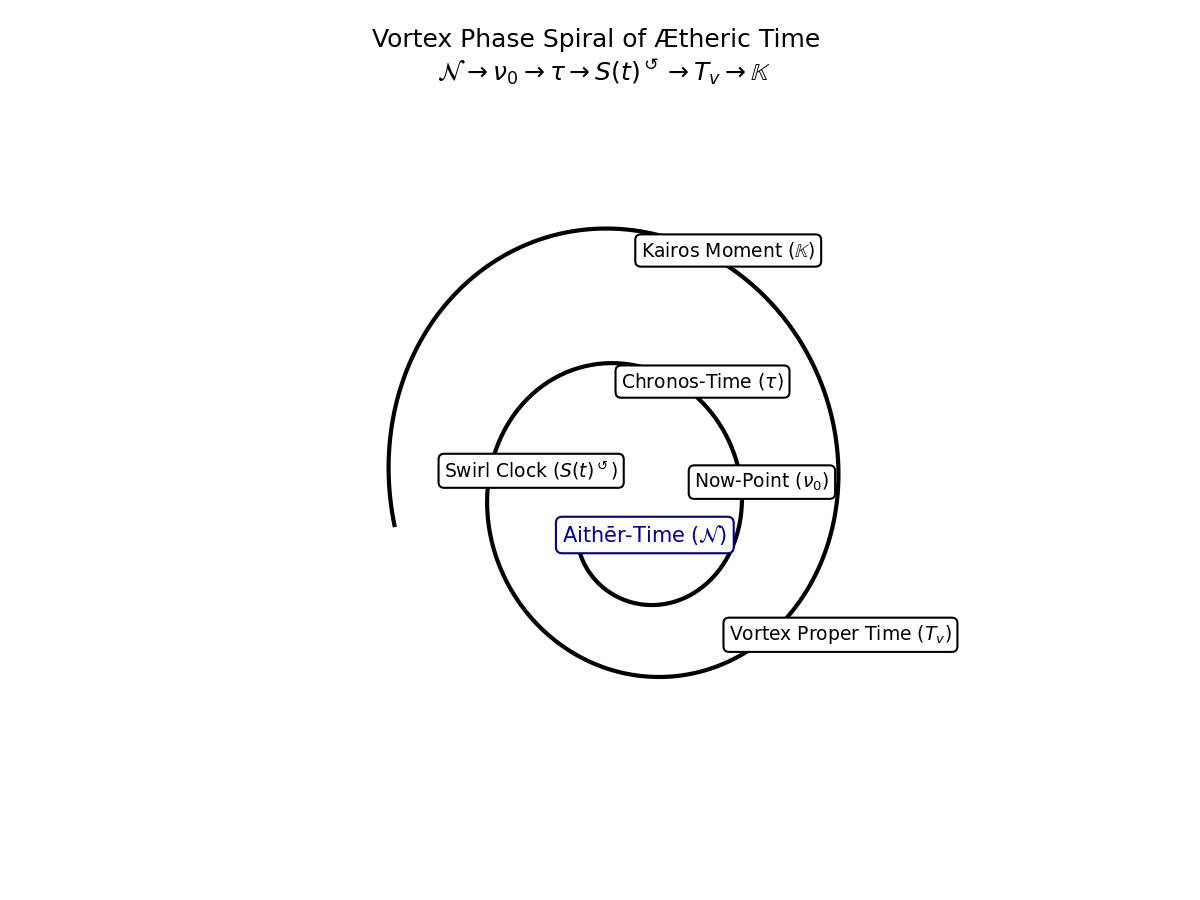
\includegraphics[width=0.7\textwidth]{images/TemporalOntologyv2}
    \caption{Temporal ontology in the Vortex Æther Model. Each layer represents a distinct phase of time, with the æther time $N$ as the absolute global parameter. The now-point $\nu_0$ defines local simultaneity, while observer time $\tau$ and swirlclock phase $S(t)$ emerge from structured vorticity.}
\end{figure}

\begin{table}[H]
\centering
\renewcommand{\arraystretch}{1.1}
\begin{tabular}{|l|l|l|}
\hline
\textbf{Symbol} & \textbf{Name} & \textbf{Interpretation} \\
\hline
$N$ & \textbf{Æther time} & Absolute global evolution parameter \\
$\nu_0$ & \textbf{Now-point} & Local simultaneity surface \\
$\tau$ & \textbf{Observer time} & Proper time: dependent on swirl density \\
$S(t)$ & \textbf{Swirlclock phase} & Emergent causal time: $\int \Omega_\text{swirl} dt$ \\
$T_v$ & \textbf{Vortex time} & Internal cycle time of knotted circulation \\
$\mathbb{K}$ & \textbf{Kairos moment} & Critical topological transition event \\
\hline
\end{tabular}
\caption{Temporal layers in the Vortex Æther Model (cf. Section 2.3 in \cite{iskandarani2025vam2}).}
\end{table}

\subsection*{Connection to Swirlclock Dynamics}

Our derivations of neutrino oscillations and $T$-violation are rooted in this ontology. In particular:

\begin{itemize}
    \item The \textbf{phase lag} $\Delta \theta_{ij}(t)$ between neutrino eigenstates directly corresponds to differential evolution in their local swirlclocks.
    \item The \textbf{vortex time} $T_v \sim 2\pi / \Omega_{\text{swirl}}$ defines the period of internal knot precession, replacing proper time in quantum oscillation models.
    \item The \textbf{observer time} $\tau$ is recovered via time dilation from vortex energy:
    \[
    d\tau = dt_\infty \sqrt{1 - \frac{U_{\text{vortex}}}{U_{\text{max}}}}, \quad
    U_{\text{vortex}} = \frac{1}{2} \rho_\text{\ae}^{(\text{energy})} |\vec{\omega}|^2.
    \]
    \item The \textbf{swirlclock-to-æther} conversion, valid across all energy scales, is:
    \[
    \frac{d\tau}{dN} = \sqrt{1 - \frac{v^2}{c^2}} \quad \text{(for uniform swirl speed)}
    \]
    or more generally,
    \[
    \frac{d\tau}{dN} = \sqrt{1 - \left( \frac{\vec{v} \cdot \vec{\omega}}{\omega_{\text{bg}} c} \right)^2},
    \]
    where $\omega_{\text{bg}}$ is the background swirl scale. This formulation links temporal flow to the energetics and orientation of vorticity fields.
\end{itemize}

This phase-based model of time aligns with the VAM temporal ontology defined over the manifold:
\[
N = E^3 \times N,
\]
where swirlclock phase $S(t)$ and vortex time $T_v$ represent emergent local and internal clock structures.

\begin{figure}[H]
    \centering
    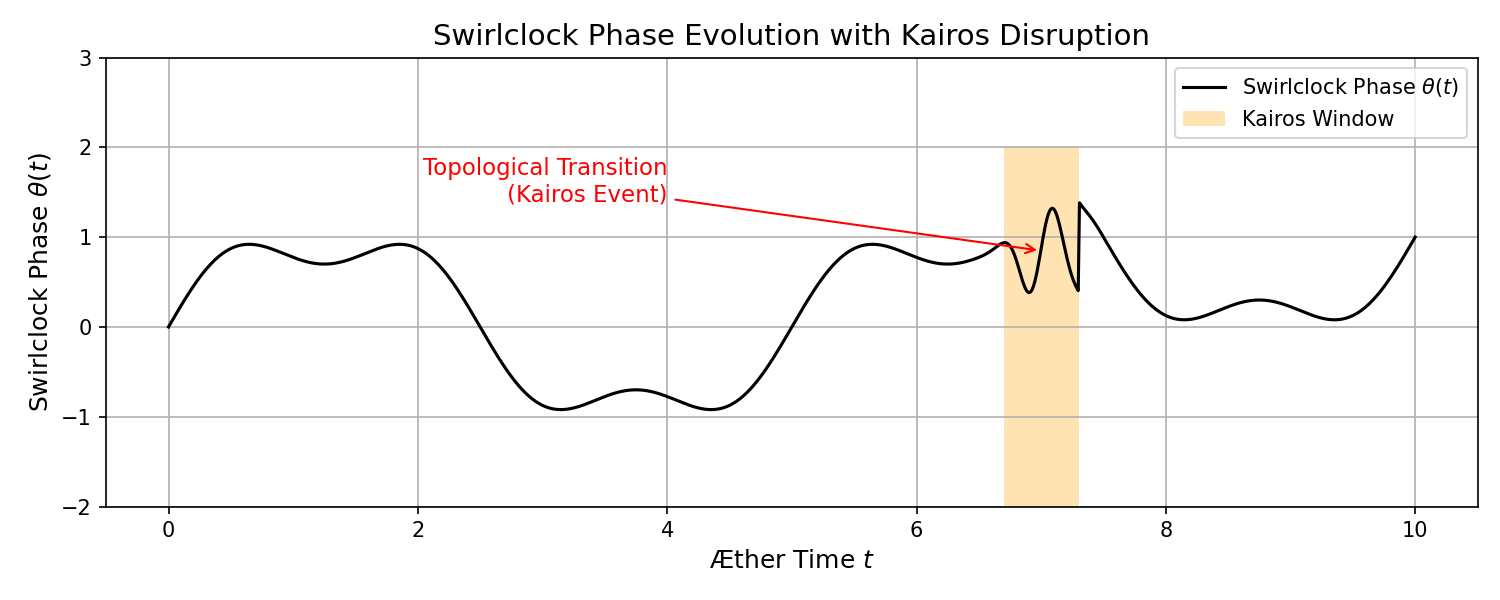
\includegraphics[width=0.7\textwidth]{images/TemporalOntologyKairosMoment}
    \caption{ Temporal ontology with Kairos moment $\mathbb{K}$ as a critical topological transition. This moment represents a discrete event where the swirlclock phase $S(t)$ and æther time $N$ align, marking a significant change in the system's state.}
\end{figure}

\subsection*{Topological Time Asymmetry}

The temporal asymmetry observed in kaon and neutrino oscillations becomes geometrically natural under VAM. Because mirror knots are not smoothly deformable into their counterparts under $T$-reversal:
\[
T: \theta(t) \rightarrow -\theta(-t),
\]
topological chirality introduces an intrinsic arrow of time. Matter--antimatter imbalance thus results not from arbitrary CP-violating phases but from topological swirlclock bias seeded during vortex formation in the early æther.

\subsection*{Conclusion}

This work aligns fully with the Temporal Ontology laid out in the foundational VAM documents. Swirlclock dynamics, topological chirality, and internal phase structure together yield an emergent model of time in which causal asymmetry, quantum oscillations, and gravitational dilation all arise from structured vorticity.

This lays the groundwork for a fully fluid-dynamical replacement of both spacetime curvature and complex Hilbert phase evolution in modern physics.
